% Preamble
\documentclass{hnu}

% Packages
\usepackage{amsmath}
\usepackage{graphicx}
\usepackage{overpic}
\usepackage{fontspec}
\usepackage{multirow}
\usepackage{subfigure}
\usepackage{enumitem}
\usepackage{booktabs}
\usepackage{multirow}
\usepackage{amssymb}
\usepackage{float}
\usepackage{setspace}
\usepackage{pkgs/cover}
\usepackage{pkgs/copyright}
\usepackage{pkgs/tocloflot}
\usepackage{pkgs/bibliography}
\usepackage{pkgs/appendix}


% 将所有 itemize/enumerate 的 topsep 调成 \parskip,其它间距清零
\setlist[itemize,enumerate]{
  topsep=\parskip,    % 列表与前后段落的垂直间距
  partopsep=0pt,      % 列表环境额外间距
  parsep=0pt,         % 列表内部段落间距
  itemsep=0pt         % 条目之间的间距
}

% Document
\begin{document}
    \createCover % 封面

    \frontmatter
    \createCopyright % 版权

    % ========================================摘要部分
    \begin{abstractCN}
测试

\keywordsCN 测试
\end{abstractCN}

\begin{abstractENG}
test

\keywordsENG test
\end{abstractENG}
    % ========================================摘要部分

    \createTOC % 目录
    \createLOF % 插图索引
    \createLOT % 附表索引

    \mainmatter
    % ========================================正文部分
    \chapter{绪论}
\vspace{7pt}

\section{研究背景与目的}
图\ref{fig:test}测试了插图效果:
\begin{figure}[H]
    \centering
    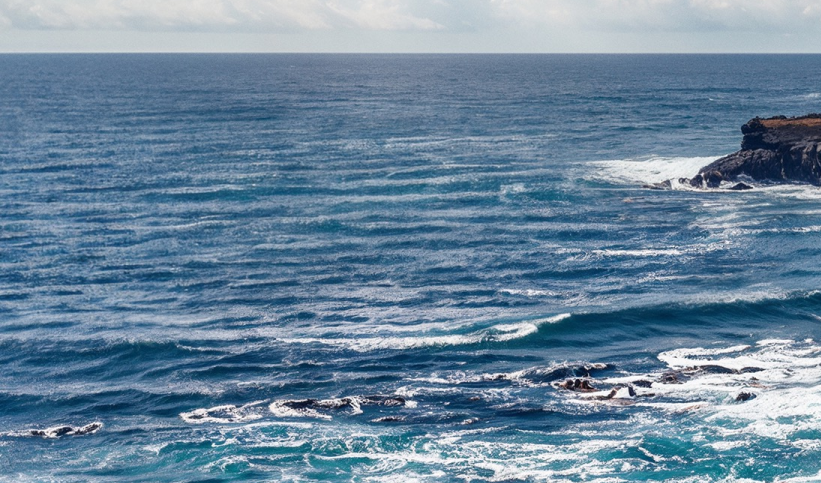
\includegraphics[width=0.75\linewidth]{src//docs//imgs/test.png}
    \caption{图名测试}
    \label{fig:test}
\end{figure}

表\ref{tab:debug_types}测试了插表效果。
\begin{table}[ht]
    \abovetopsep=0pt
    \aboverulesep=0pt
    \belowrulesep=0pt
    \belowbottomsep=0pt
    \begingroup
    \centering
    \caption{表名测试}
    \label{tab:debug_types}
    \fontSimsun\sizeFive
    \newcolumntype{Z}{>{\centering\arraybackslash}X}
    \begin{tabularx}{\textwidth}{Z|Z}
        \toprule
        类型 & 描述 \\
        \hline
        1 & 2 \\
        \hline
        3 & 4 \\
        \hline
        \bottomrule
    \end{tabularx}
    \endgroup
    \vspace{3pt}
\end{table}

\section{研究内容与挑战}

研究面临以下挑战:
\begin{itemize}
  \item TEST1
  \item TEST2
\end{itemize}

本文其余章节安排如下:\hyperref[Related work]{第二章相关工作}综述了XXX
    \chapter{相关工作}\label{Related work}

本章将综述与本研究相关的既有工作,主要涵盖 XXX

\section{XXX研究}
为在 TrustZone 提供的基础隔离之上实现更精细化的安全控制,Brasser 等人\cite{brasser_sanctuary_2019} 提出了 SANCTUARY,旨在为用户态受信应用提供与 Intel SGX 相似的硬件隔离机制。SANCTUARY 的工作体现了在 TrustZone 框架下构建更强安全边界的尝试。

Zhang 等人\cite{zhang_shelter} 提出的 Shelter 即为一例。该工作扩展了 Arm 的 机密计算架构(Confidential Compute Architecture, CCA),为用户态应用提供硬件隔离,反映了 Arm 为更广泛应用场景提供硬件级安全保护的发展趋势。

\section{YYY研究}

\section{ZZZ研究}

\section{其他工作}

    % ========================================正文部分

    % 参考文献
    \createBibliography    

    % ========================================致谢部分
    \begin{newThanks}
麓山巍巍,湘水泱泱。宏开学府,济济沧沧。承朱张之绪,取欧美之长,华与实兮并茂,兰与芷兮齐芳。楚材蔚起,奋志安攘。振我民族,扬我国光。
\end{newThanks}

    % ========================================致谢部分

    % 附录
    \createAppendix
    % ========================================附录部分
    \chapter{关键代码}\label{Code}
\vspace{0.5cm}

\begin{lstlisting}
#define DBGKEY                                       0xA05F
#define C_DEBUGEN                                  (1 << 0)
#define C_HALT                                     (1 << 1)
#define C_STEP                                     (1 << 2)
#define C_MASKINTS                                 (1 << 3)
#define S_HALT                                    (1 << 17)
#define M4_DHCSR_ADDR        (volatile uint32_t*)0xE000EDF0
#define M4_CPUID_base_register        (uint32_t*)0xE000ED00
\end{lstlisting}
    % ========================================附录部分
    
\end{document}
